\chapter{Implementation}
\label{chapter:implementation}

The architecture of the application contains two main modules: the user interface (UI) in the form of a Web Application, presented in \autoref{sec:impl-wa} and the actual implementation of the conversational agent, detailed in \autoref{sec:impl-conversational-agent}.

In the next sections reference to the chat client, chat server and chat-bot signify the front end user interface, the back end of the web application and the conversational agent program respectively.

\section{Web Application}
\label{sec:impl-wa}

The web application is the interface with the help of which the user interacts with the conversational agent. It implements a chat client, a program where the user can input its questions and see the answers processed by the conversational agent and returned by the chat server. It also implements a chat server that connects to the chat-bot's endpoint. After the connection succeeds, the chat server passes the query received from the client to the chat-bot, waits for a reply and then sends the reply back to the client.

The chat client is described in \autoref{sub-sec:impl-wa-front-end} and the chat server is described in \autoref{sub-sec:impl-wa-back-end}. The chat-bot's endpoint of the aforementioned connection between him and the chat server is explained at large in \autoref{sec:impl-conversational-agent}.

\subsection{Front End}
\label{sub-sec:impl-wa-front-end}

The front end is written in HTML, CSS and JavaScript and it is composed of two main screens: the first page where the user can input the name of the personality he wishes to speak to; the second page, the actual chat box, where the conversation is displayed, and the input box, where the user can write the question and submit it.

The first screen is shown in \autoref{fig:web-app-first}. Clicking the {\em Enter} button would send a request to the chat server that would later on initialize the chat-bot with the inputted personality.

\begin{figure}[htb]
  \centering
  \captionsetup{justification=centering}
  
\includegraphics[width=\textwidth]{src/img/web-app-first.png}
  \caption[Web Application - First Window]{The first page of the Web App where the user can input the name of the personality he wants to talk with}
  \label{fig:web-app-first}
\end{figure}

In \autoref{fig:web-app-second}, the chat box containing a few questions and answers can be seen. At the bottom of the chat box there is the input text box where the user can write its questions and submit them.

\begin{figure}[htb]
  \centering
  \captionsetup{justification=centering}
  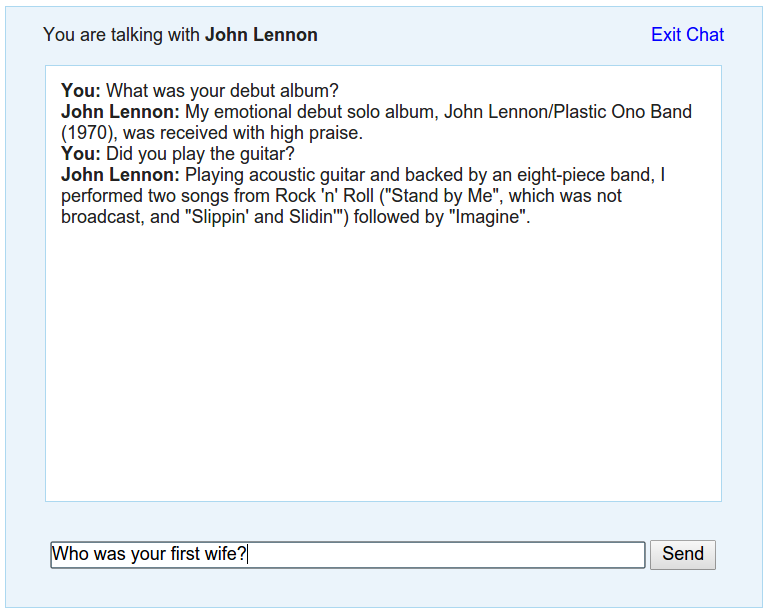
\includegraphics[width=\textwidth]{src/img/web-app-second.png}
  \caption[Web Application - Second Window]{The page where the user can submit questions and see the replies}
  \label{fig:web-app-second}
\end{figure}

The conversation is saved on the client-side, in memory, using JavaScript, and is persistent until the page is refreshed or closed.

The questions are submitted by sending a synchronous HTTP GET request to the server. The request contains the question. The request is sent using AJAX (Asynchronous JavaScript + XML) and contains a random generated number in the URL so that the browser doesn't serve a cached page. For example, \url{http://<hostname>/chatbot.php?question=What+was+your+debut+album\%3F\&t=0.023473239736631513} sends the question {\em "What was your debut album?"} to the chat server.

\subsection{Back End}
\label{sub-sec:impl-wa-back-end}

The server side of the web application is made up of XAMPP\footnote{\href{https://www.apachefriends.org/index.html}{XAMPP Website}\url{https://www.apachefriends.org/index.html}}\textsuperscript{,}\footnote{XAMPP is a bundle containing the Apache HTTP server, a MySQL server and a PHP and Perl interpreter} and the PHP scripts that implement the connection with the chat-bot.

Functionally, the communication is accomplished by using a local socket to socket connection between the web server and the conversational agent server. A snippet of the code the shows the principles of communication between the two servers is presented in \autoref{lst:backend}. The main aspects of the program are highlighted through comments in the code. The flow of the communication is shown in \autoref{fig:client-server-flow}.

\lstinputlisting[language=PHP, firstline=11, lastline=32, caption=Socket communication between the web server and the chat-bot, label=lst:backend]{src/code/chatbot.php}

\begin{figure}[htb]
  \centering
  \captionsetup{justification=centering}
  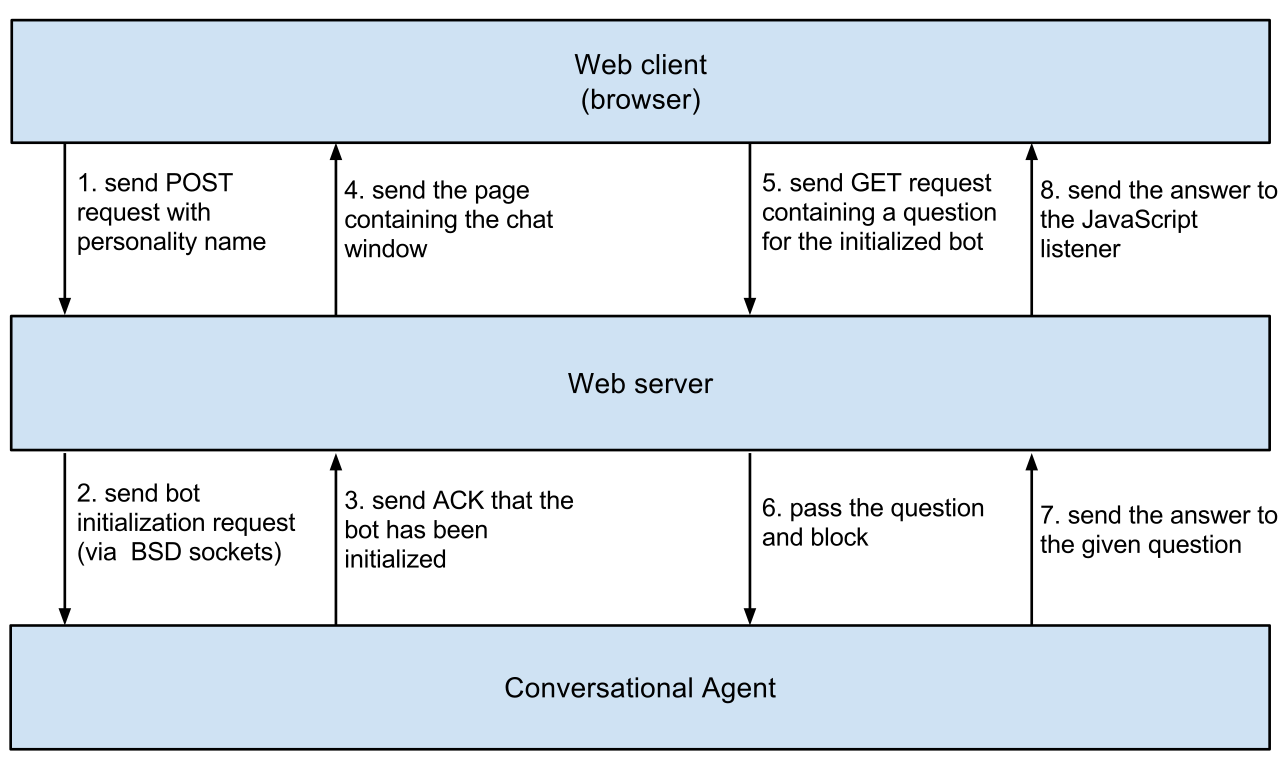
\includegraphics[width=\textwidth]{src/img/client-server-flow.png}
  \caption{The communication flow between the client, web server and conversational agent server}
  \label{fig:client-server-flow}
\end{figure}


\section{Conversational Agent}
\label{sec:impl-conversational-agent}

This section contains the architectural decisions and the implementation details of the conversational agent. First, in \autoref{sub-sec:impl-ca-rule-based}, the  rule-based system approach using the DBpedia ontology and the ChatScript engine is described. Next, the approach to implementation employing the {\em answer sentence selection} method is presented.

\subsection{Rule-based System Approach}
\label{sub-sec:impl-ca-rule-based}

Expressing a Property
In order to understand what is trying to be expressed in a
sentence, we start from the DBpedia properties of a large
set of people. Subsequently, for every property, we try to
determine how that property is expressed in the Wikipedia
corpus. For the information extraction, we use Stanford
CoreNLP.
To find the manner in which a property is expressed, we
searched the value of that property in the sentences from
Wikipedia where the person which the article is about
appears in. Having the desired sentence identified, we
annotated it using Stanford CoreNLP and obtained a
syntactic parse tree. Analyzing this tree, we determined that
the root is the verb directly connected with the subject.
Having the parse tree, we considered that the best way to
express the property is the path from that property to the
root verb.
Applying this algorithm to a large set of people, we
managed to build a big, but extensible knowledge base by
introducing the most relevant output expressions in a
knowledge base.

Pattern Generation
In order to generate ChatScript files for a specific person, we fetch that person's Wikipedia page, split it into phrases and keep only those that have the person as a subject. This filtering was done using the Stanford Deterministic Co-reference Resolution System. After extracting all the phrases referring a the current historical figure, we select only those that express a property from DBpedia matching the expression against the knowledge base. We then create a rule-answer entry to add to the ChatScript files. The rule is represented as an expression of a property that appears both in the analyzed sentence and the knowledge base. The answer is the analyzed sentence from Wikipedia which is converted to be expressed in the first person. The conversion from the third person to the first person of the sentence is accomplished with Stanford's Part-of-Speech Tagger and CoreNLP. All these patterns are written in ChatScript's file hierarchy. For a fast and easier way to find the answer, we arranged ChatScript's files by the properties of the person.

\subsection{Answer Sentence Selection Approach}
\label{sub-sec:impl-ca-ass}

Because it is impossible to build an exhaustive rule-based system, a secondary approach to this problem has to be taken into consideration in order to give a good answer. In addition, ChatScript has its own limitations coming from the fact that it ignores a rule after it first matches it. Therefore a fallback option is needed in case the former approach fails to provide an answer.
Considering the fact that the former approach gives better answers the simpler and more common questions are asked, we observe that either it fails to match questions that are more complex or it has to many matches for a question that uses a common verb (like “to be” or “to have”) and the results will be inaccurate or noisy. The solution to avoid this is to try and find the answer directly from the source of the previously described knowledge base with an ad hoc approach considering every sentence from that respective source.

Following the goal of having to answer a question for a certain historical figure, the set of possible answers is reduced to a set of sentences from that person's biography.
This leaves us with the task of identifying a sentence from a biography that has the highest probability of correctly answering the question at hand.
Considering what was previously stated, that this approach tries to find the answer to a more complex question, we can assume, at least for now, that there is a great deal of semantic information embedded in the form of the question (lexically and semantically) so that the chances are a part of the answer textually lies in the question. Therefore, what we can do is actually search for the question (or paraphrases of the initial question) in the reference text.

The design of this approach is built with three main goals in mind: performance regarding speed, small memory footprint and high answer accuracy.

{\em Speed.} Good speed efficiency is achieved by using a pipeline architecture, where the set of potentially correct answers is iteratively reduced as the methods for sentence selection increase in complexity. This pipeline can be viewed as a series of sieves that sequentially filter the set of input sentences. The pipeline architecture is discussed in depth in \autoref{sub-sub-sec:pipeline}. In addition, the use of Lucene's in-RAM storage (described in \autoref{sec:lucene}) saves a lot of time from accessing persistent storage devices (HDD, SSD etc.). More than that, all tools used are highly optimized and no extra features of these tools are integrated in the program if not necessary.

{\em Memory.} By not using a rule-based system, there is no need for huge databases stored on the hard-drive. Also, if the program has internet access, the pages needed for information retrieval can be fetched immediately from the Web. Although, if this is not possible, the biographical corpus used by the agent can be scaled according to the desired set of people the program could potentially instantiate. Regarding the RAM memory, the efforts to minimize the memory footprint are backed by:

\begin{itemize}
  \item the optimized indexing of Apache Lucene
  \item the control of Stanford CoreNLP annotations
  \item the Java language references support (by not duplicating paragraphs or sentences)
  \item using hard-drive stored dictionaries for WordNet
\end{itemize}

{\em Answer accuracy.} The "correctness" of the answers is achieved through the scoring method of the selected sentences, using both Lucene's internal scoring system and own formulas for scoring sentences according to the score of the paragraphs and WordNet's frequency count for the synonyms considered in the alternative formulations of the input question.

The class diagrams for the program can be seen in \autoref{chapter:class-diagrams}.

\subsubsection{Pipeline}
\label{sub-sub-sec:pipeline}

\begin{figure}[htb]
  \centering
  \captionsetup{justification=centering}
  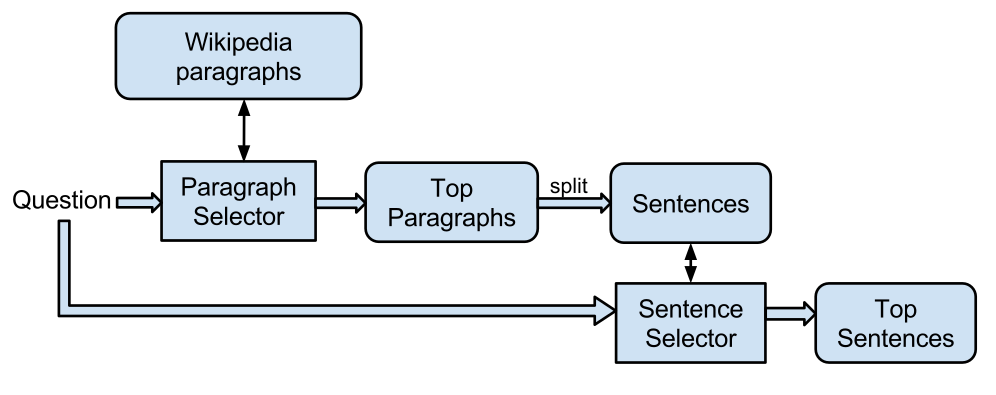
\includegraphics[width=\textwidth]{src/img/pipeline-lexical.png}
  \caption{The lexical filtering part of the pipeline}
  \label{fig:pipeline-lexical}
\end{figure}


Answer sentence selection

To get the best results out of this approach, we need to follow a number of steps.
First, we need to remove unnecessary words, including stop words, the interrogative words (what, when, where, who, why and how) and irrelevant verbs (“to be”, “to have” and other similar verbs as described above) in order to remain only with meaningful words, i.e. the kernel of the question.
Second, we want to use the Stanford CoreNLP software to lemmatize the question (i.e. to convert every word to its appropriate canonical form) because, as described later on, the corpus used for a historical figure will be lemmatized too. This will help in the search step because words will more likely match if they are in their base form.
Third, we try to find alternative ways of expressing the input question and attempt to search for all this variants in the biographical text. We do this by trying different synonyms for the words in the question so that we can get more results, even if the initial question is formulated in such a way that it does not contain the exact words that might appear in the sentence representing the correct answer.
Next, the top paragraphs from the Wikipedia article are filtered based on the textual matching score between the question and the respective paragraph given by Apache Lucene [1], a text search tool. Then, we apply the same algorithm at the level of sentences instead of paragraphs. In short, to get the best answer the corpus is divided in separate paragraphs and a small set of paragraphs where the answer sentence might be part of are selected. Next, we attempt to find an even smaller set, made of sentences that are the best candidates to answer the question.
After we have a set of sentences that passed the lexical filtering, we want to eliminate those in which the subject of the sentence does not match the subject of the question. These mechanism is similar to maintaining the semantic relations as described in [5], and presented above in the Related Work section. To achieve that, we want to use Stanford CoreNLP, and in particular the Stanford Deterministic Co-reference Resolution System, to determine who is the subject of a given sentence.
After the syntactic filtering we are left only with the semantic filtering. This means we want to filter out all the sentences that do not have the type as the one expected by the question. For example, questions starting with “When” expect a answer sentence that contains a numerical value.
Finally, we choose the first sentence in order of the previously gathered relevance scores. Using the aforementioned approach we manage to answer more complex questions.

\section{Testing}
\label{sec:testing}
